% Compile with pdfLaTeX from Docs/report/.
% Figure paths match auxiliary_feature_summary.tex.
\documentclass[11pt]{article}

\usepackage[margin=1in]{geometry}
\usepackage{booktabs}
\usepackage{amsmath}
\usepackage{graphicx}
\graphicspath{{images/}{../../images/}{../../}}
\usepackage[font=small,skip=2pt]{caption}
\usepackage[hidelinks]{hyperref}
\usepackage{tikz}
\usetikzlibrary{arrows.meta}

\title{Predicting HDB monthly rent from past information}
\author{}
\date{October 2026}

\begin{document}
\maketitle

\begin{abstract}
Labelled approvals run from January 2021 through March 2025.
They are divided by approval month into a training set, through September 2024, a validation set, October through December 2024, and a test set, January through March 2025.
Only the validation set is used to stop or choose a model.
The test set is scored after that choice and does not enter it.
The unlabelled months after March 2025 are the private test set, and its score is not used to stop or choose a model either.
Features for an approval month therefore may not use the true rents of later months, or later economic series such as COE premiums and stock prices.
The scored prediction is a town-month mean of rent per square metre, a within-town gap from that mean, and one shared network that turns those pieces into monthly rent.
On the private test set the submitted predictions have RMSE 451.26.
\end{abstract}

\section{Introduction}
\label{sec:intro}

The prediction target is \texttt{MONTHLY\_RENT}.
The labelled approvals run from January 2021 through March 2025 and are divided by approval month into three sets.
The training set is every month through September 2024.
It is the only set used to fit parameters.
The validation set is October through December 2024.
It is the only set used to stop or choose a model.
The test set is January through March 2025.
It is scored after that choice and does not enter it.
The private test set is the unlabelled table after March 2025.
Its RMSE is not used to stop or choose a model.
A feature for an approval month may use only information already known before that approval.
The project does not train an attention model.
The constraint is only that the true rent path after the month being predicted is not an input.

Two constructions enforce the rule in the feature table.
The six group-mean columns use labelled rents from the previous three approval months only.
No other auxiliary column reads \texttt{MONTHLY\_RENT}.
The region model is a recurrent network, one per town.
For the month being predicted it uses the time index and the economic trend already observed before that month.
It does not receive that month's true rent, a previous predicted rent, or the true town-month rents of later months.
Earlier economic inputs are carried by the hidden state.
The sequence is started in 2021 so that the state already exists when a later month is predicted.

The multistage prediction follows from that split of information.
The recurrent network first traces the town's unit-price path, the movement shared by flats in the same town.
A flat's own location and attributes then explain how far its unit price sits from that path.
A final network combines the path, that gap, and the flat's other numbers into one monthly rent.

\section{Source-column preprocessing}
\label{sec:source}

The raw labelled table and the private test set are left unchanged.
Eleven derived columns are written into the auxiliary table, and the same maps are applied to both.
None of them reads \texttt{MONTHLY\_RENT}.

Each column keeps the transform that matches its kind.
\texttt{approval\_month\_index} is the number of months since January 2021: September 2024 is 44 and July 2026 is 66.
\texttt{lease\_commence\_year} stays a four-digit year and is not turned into a month index.
\texttt{town\_key}, \texttt{block\_key}, and \texttt{street\_key} strip, lowercase, and collapse spaces.
They are names, not price ranks.
The feature \texttt{block\_key} is the normalized block identifier only.
The \texttt{BLOCK}$|$\texttt{STREET} string used to join the block table is a separate key and is not stored as this feature.

\texttt{flat\_type\_ord} turns hyphens into spaces and maps 1-room through 5-room to 1 through 5 and executive to 6.
Median floor area rises along that order, from about 31 square metres for a 1-room flat to about 144 for an executive flat.
The rank is that size order.
It is not estimated from rents in later approval months.
\texttt{flat\_model\_ord} is a fixed rank from 0 through 19, ordered from cheaper to dearer names in the labelled table.
\texttt{flat\_model\_key} keeps the normalized name as a category, so a tree can split on a subset of names.
The mixture and the numeric network receive only the rank.
The labelled table has 20 names.
The private test set has 19 of them and no name that is absent from the labelled table.
\texttt{4-room} and \texttt{4 room} become the same type, and a street in the private test set such as \texttt{Whampoa Drive} matches the lowercase streets of the labelled table after this normalization.

\texttt{floor\_area\_sqm} and \texttt{fee\_amount} stay floats and are not standardized on the whole table.
\texttt{furnished\_bin} is 1 for yes and 0 for no.
\texttt{FURNISHED} is yes on every labelled row and every row of the private test set, and \texttt{FEE} is 0 on every row, so those two fields do not vary.

\section{Auxiliary features}
\label{sec:auxiliary}

The auxiliary table has 94 columns, kept in the same row order as the rental records.
Labelled rows and the private test set are joined back by that order and are not sorted.
The auxiliary files do not share the rental row key.
Stations, schools, and malls have coordinates but no block number.
The block table is the hub: it has both an address and coordinates, and every later spatial column starts from that join.
Block, distance, COE, and stock columns do not read \texttt{MONTHLY\_RENT}.
Distances are Haversine kilometres with Earth radius 6{,}371\,km.
The figures below describe the constructed columns.

\subsection{Block attributes and age}

The rental row is left-joined to the block file on
\begin{equation}
\texttt{block\_key}
=
\mathrm{norm}(\texttt{BLOCK})
\mathbin{\Vert}
\mathrm{norm}(\texttt{STREET}),
\end{equation}
where \texttt{norm} strips, lowercases, and collapses spaces, and letters inside \texttt{BLOCK} are kept.
The key matches all 150{,}000 labelled rows and all 50{,}000 rows of the private test set, and the row count does not change.
The copied fields are latitude, longitude, postal code (\texttt{NIL} becomes null), maximum floor, year of completion, subzone, planning area, and region.
Building age is the approval year minus the completion year.
Lease age uses \texttt{LEASE\_COMMENCE\_DATE} instead.
A third column is the gap between those two years, and a product of building age with a Central Region flag lets a linear model treat age differently in the centre.
Town alone does not say whether the block is central, new, or tall, and the same completion year is a different age in 2021 and in 2026.
Figure~\ref{fig:blocks} shows the joined region and those age and floor distributions.

\begin{figure}[ht]
\centering
\begin{minipage}[t]{0.38\textwidth}
\centering
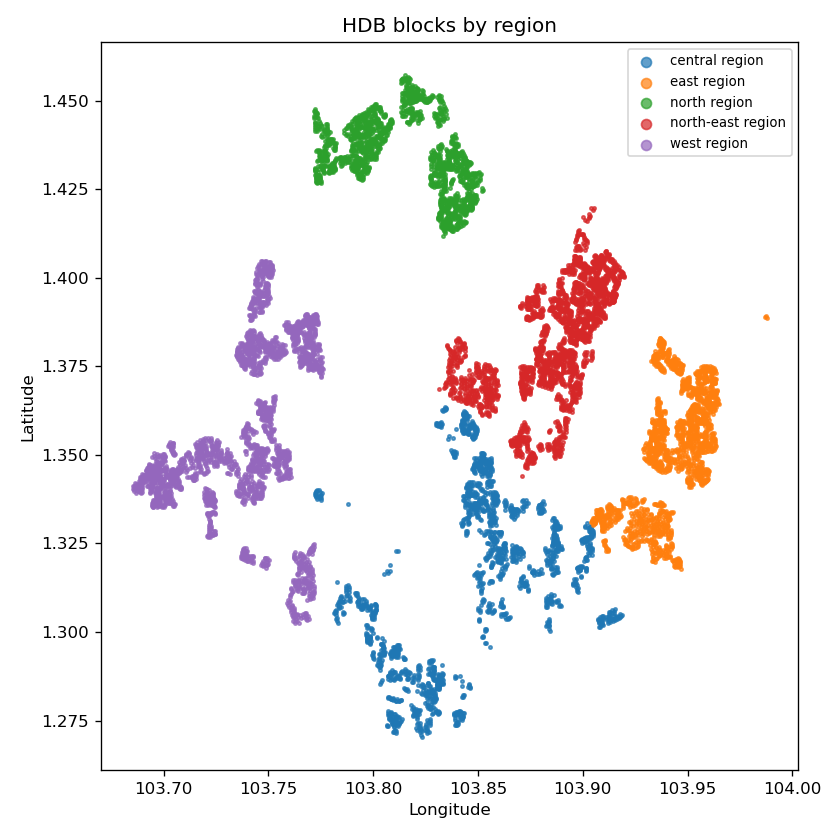
\includegraphics[width=\linewidth]{images/blocks_region_map.png}\\[0.2em]
{\small (a) Region after the address join.}
\end{minipage}\hfill
\begin{minipage}[t]{0.56\textwidth}
\centering
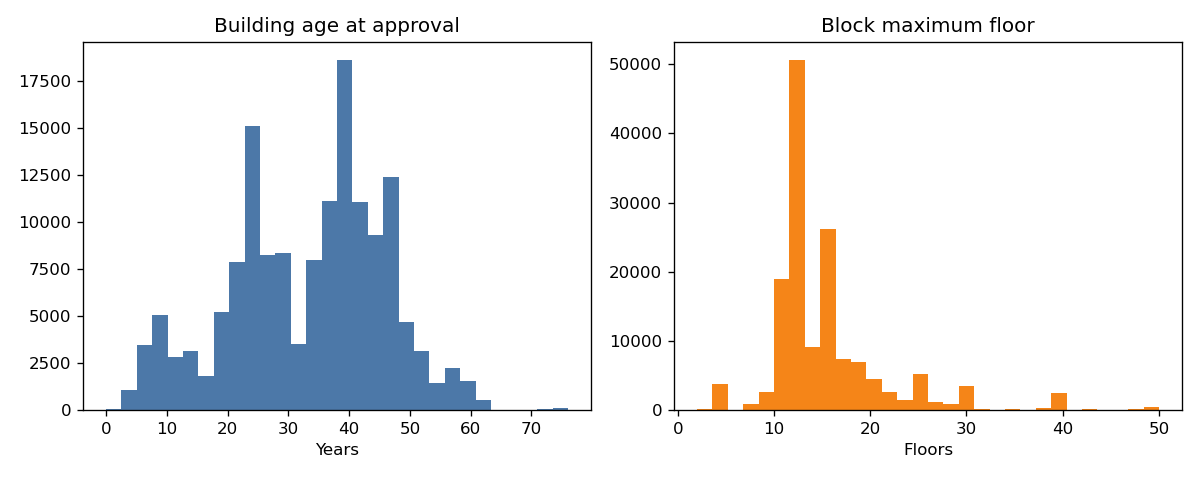
\includegraphics[width=\linewidth]{images/blocks_age_floor.png}\\[0.2em]
{\small (b) Age at approval, and maximum floor.}
\end{minipage}
\caption{Block attributes copied onto the rental rows.}
\label{fig:blocks}
\end{figure}

\subsection{MRT}

The open trunk set is stations with status \texttt{open} whose code prefix is NS, NE, CC, DT, TE, EW, or CG.
The two open Changi Airport (\texttt{CG}) stations are labelled EW.
For each block the table stores the nearest trunk station's distance, code, normalized name, and line, the nearest station and distance on each of the six lines, and the number of trunk codes within 0.5, 1, and 2\,km.
Ties closer than $10^{-6}$\,km keep the lexicographically smallest code.
Planned stations, and prefixes CR, JE, JS, JW, and CP, stay in their own distance columns so they cannot shrink the open-station distance.
A flag is 1 when the nearest trunk station's name has at least two codes.
The motivation is access: a flat near a station is easier to commute from, one distance cannot tell which corridor that station serves, and a count separates a single station from a cluster.
Figure~\ref{fig:mrt} shows that most rentals are within about 1\,km of some trunk station, that 0.5\,km is often empty, and that the North East Line is farther than the East--West Line.
The MRT file has no opening date, so a station marked open may have opened after January 2021.
About 20 longitudes have only one to three decimal places.
Great-circle distance is not walking time.

\begin{figure}[ht]
\centering
\begin{minipage}[t]{0.48\textwidth}
\centering
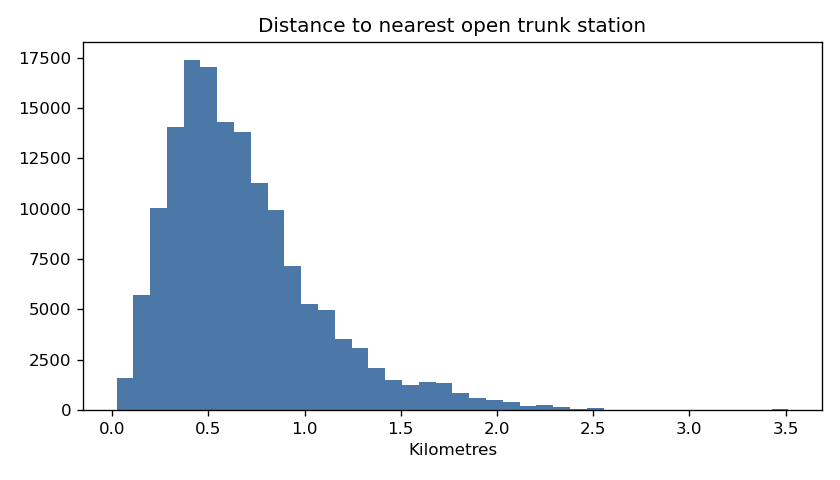
\includegraphics[width=\linewidth]{images/mrt_nearest_trunk.png}\\[0.2em]
{\small (a) Nearest open trunk station.}
\end{minipage}\hfill
\begin{minipage}[t]{0.48\textwidth}
\centering
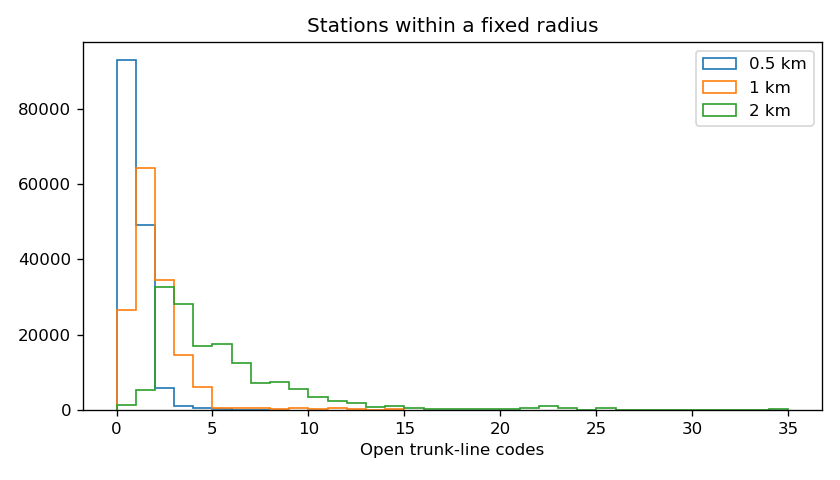
\includegraphics[width=\linewidth]{images/mrt_radius_counts.png}\\[0.2em]
{\small (b) Trunk-line codes within 0.5, 1, and 2\,km.}
\end{minipage}\\[0.6em]
\begin{minipage}[t]{0.58\textwidth}
\centering
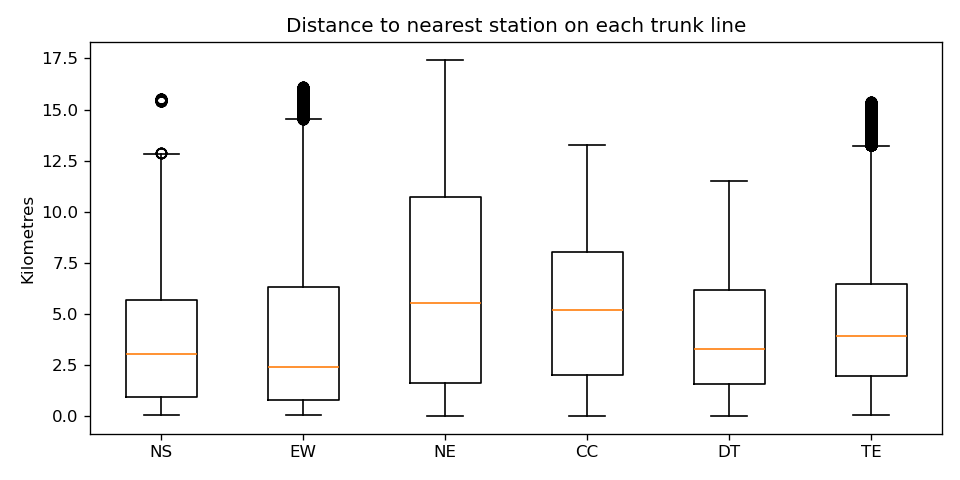
\includegraphics[width=\linewidth]{images/mrt_line_distances.png}\\[0.2em]
{\small (c) Nearest station on each trunk line.}
\end{minipage}
\caption{MRT access. An interchange is counted once per code.}
\label{fig:mrt}
\end{figure}

\subsection{Schools and malls}

Primary schools are rows with \texttt{MAINLEVEL\_CODE} equal to \texttt{primary} (179 schools).
Secondary schools are the two strings \texttt{secondary (s1-s5)} and \texttt{secondary (s1-s4)} (133 schools).
Each set contributes a nearest distance, the normalized school name, and a count within 1\,km; primary schools also have a 2\,km count.
All 337 schools add one more nearest distance, name, and 1\,km count.
All 113 malls contribute the nearest distance, normalized name, and counts within 1 and 2\,km.
Names are kept because those tables have no code, and the normalized name is unique.
Households pay for a short walk to a primary school or a shop, and a count distinguishes one neighbour from several.
Figure~\ref{fig:amenity} shows schools packed closer than malls, and many rentals with no mall inside 1\,km.
School and mall tables have no opening dates, and the school table has no university.

\begin{figure}[ht]
\centering
\begin{minipage}[t]{0.60\textwidth}
\centering
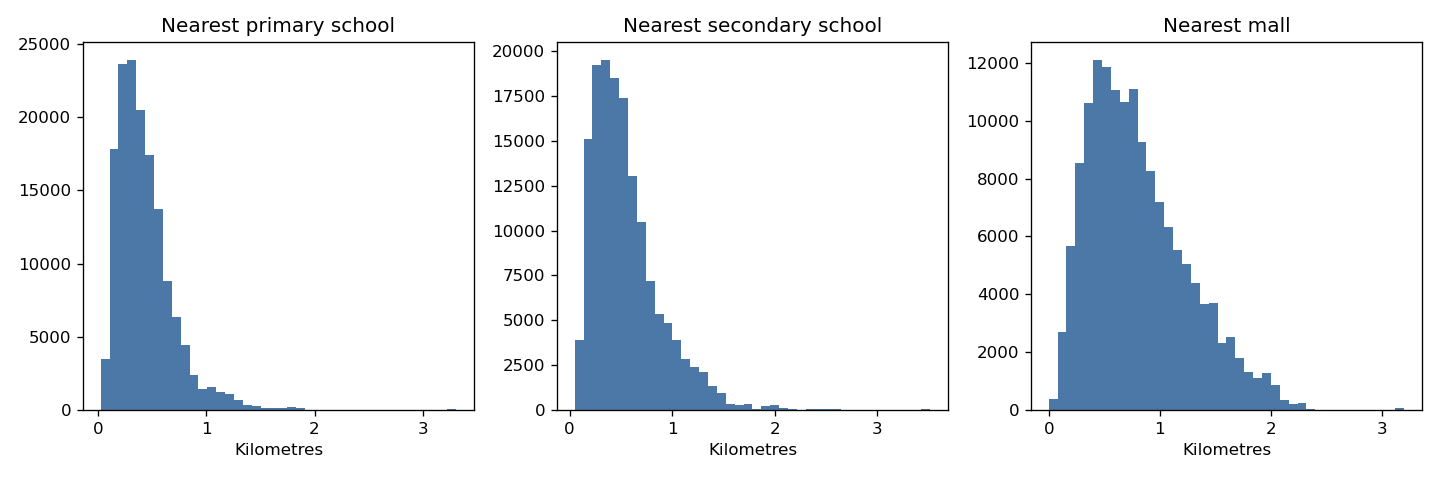
\includegraphics[width=\linewidth]{images/amenity_distances.png}\\[0.2em]
{\small (a) Nearest primary school, secondary school, and mall.}
\end{minipage}\hfill
\begin{minipage}[t]{0.36\textwidth}
\centering
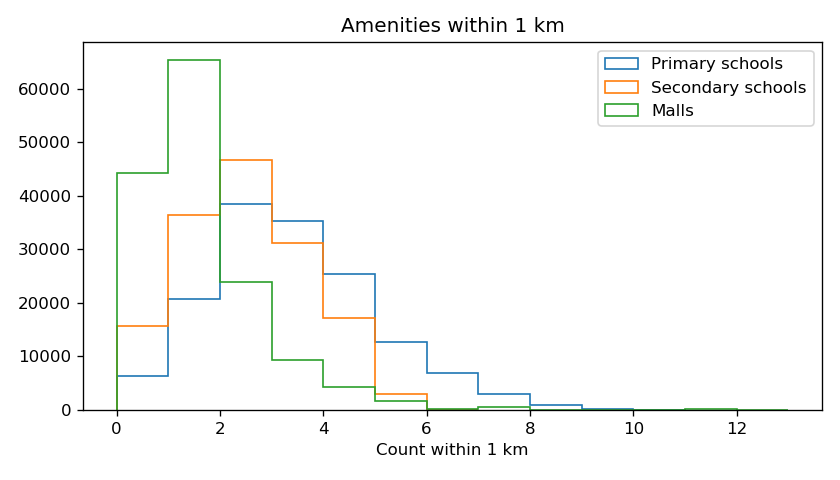
\includegraphics[width=\linewidth]{images/amenity_counts_1km.png}\\[0.2em]
{\small (b) Counts within 1\,km. Zero is a real zero.}
\end{minipage}
\caption{Schools and malls around the labelled rentals.}
\label{fig:amenity}
\end{figure}

\subsection{Density and a fixed downtown point}

The number of other HDB blocks within 500\,m uses the same block coordinates, excluding the block itself.
The town centroid is the mean latitude and longitude of blocks in that town, and each block is measured to its own centroid.
Distance to the CBD is Haversine to the fixed Raffles Place coordinate $(1.283889, 103.851389)$, taken from station codes \texttt{ns26} and \texttt{ew14}.
A log of the nearest trunk distance, $\ln(d+0.001)$, gives nearby changes more weight than a linear model would give the raw kilometres.
Two flats in the same town can still sit at the edge or next to downtown.
These density features do not use rent.
Cluster labels were not adopted: the official areas already exist, and clustering on rent would put the target into the features.

\subsection{COE and stocks}

COE amounts are parsed by stripping dollar signs and commas.
Each category-month uses bidding round 2, or round 1 if round 2 is absent.
A rental in month $T$ receives the premium, the change from $T-2$ to $T-1$, and bids divided by quota, all from month $T-1$.
Categories A, B, and E have those three columns; category A also has the mean of $T-1$, $T-2$, and $T-3$; category C has only the lagged premium.
Stock features use month-end adjusted closes.
The bank basket is the equal-weight mean of \texttt{D05.SI}, \texttt{O39.SI}, and \texttt{U11.SI}; the property basket is \texttt{C09.SI}, \texttt{U14.SI}, and \texttt{9CI.SI}.
A month is used only when all three symbols have a close, and the rental again sees month $T-1$, both as a level and as that month's return.
Dearer car quotas or weaker bank shares may coincide with tighter household budgets, which floor area and town cannot express.
Figure~\ref{fig:market} shows that both series are constant across flats approved in the same month.
January 2021 COE lags are null because December 2020 is missing.
The property basket is missing on early labelled rows because one constituent starts later.
The four COE premiums are correlated about 0.93 with each other, so the region model in Section~\ref{sec:stack} keeps one premium rather than all four.

\begin{figure}[ht]
\centering
\begin{minipage}[t]{0.48\textwidth}
\centering
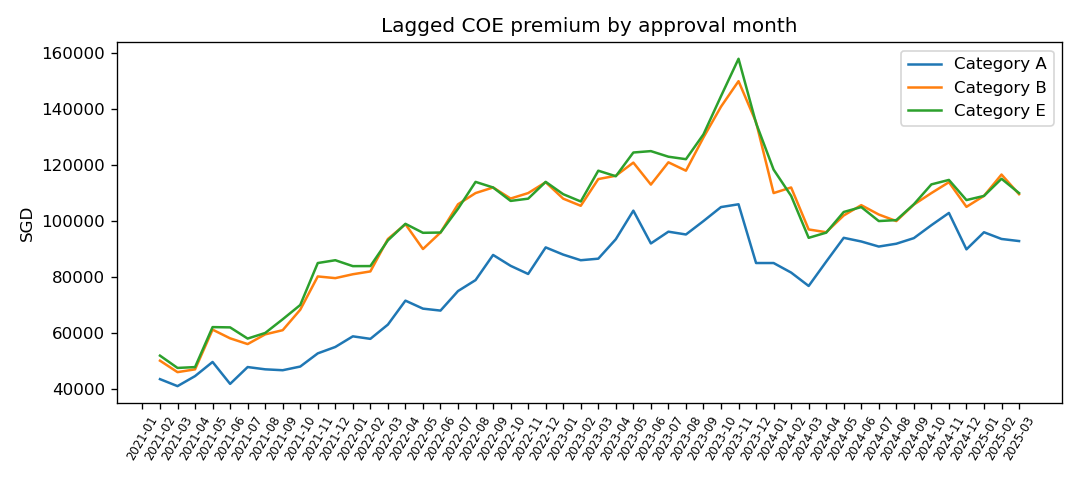
\includegraphics[width=\linewidth]{images/coe_monthly.png}\\[0.2em]
{\small (a) Lagged COE premium.}
\end{minipage}\hfill
\begin{minipage}[t]{0.48\textwidth}
\centering
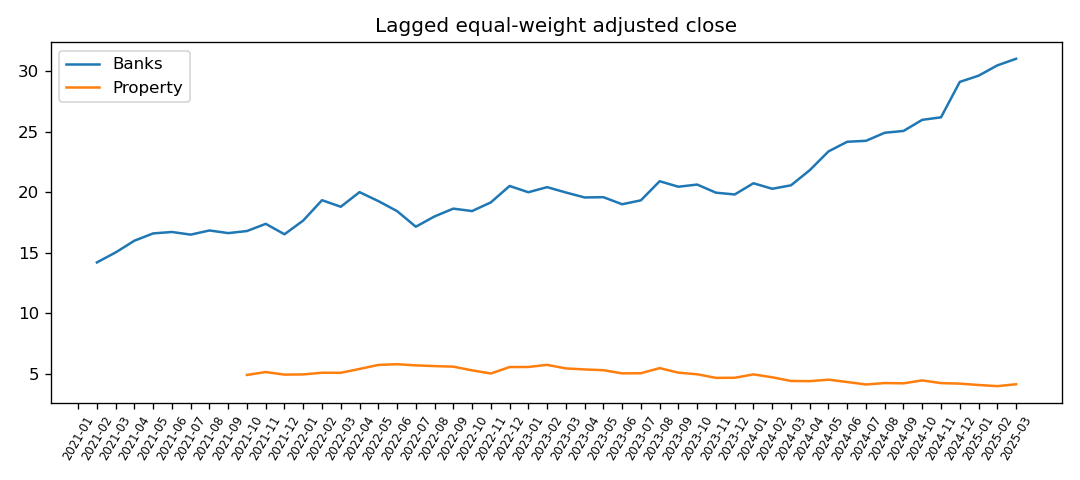
\includegraphics[width=\linewidth]{images/stock_baskets_monthly.png}\\[0.2em]
{\small (b) Lagged bank and property baskets.}
\end{minipage}
\caption{Month-level series shared by every flat approved in that month.}
\label{fig:market}
\end{figure}

\subsection{Group-mean rents}

Six columns are target encodings: smoothed mean rent by postal sector, postal district, nearest mall, nearest open MRT code, nearest primary school, and nearest secondary school.
For a row in month \(T\), only labelled rents from \(T-1\), \(T-2\), and \(T-3\) are used:
\begin{equation}
\frac{n\,\bar r_g + 20\,\bar r}{n + 20}.
\end{equation}
Here \(\bar r_g\) is the group mean inside that window, \(n\) is the number of those labelled rows, and \(\bar r\) is the island-wide mean inside the same three months.
If \(n=0\), the value is \(\bar r\).
January 2021 has none of those months in the file, so all six columns are null.
February 2021 uses January only.
Rows in the private test set never contribute rents.
The sector and district strings are not stored.
A mean accumulated since 2021 would still carry old rent levels into 2025, while the previous quarter moves with the market.
Shrinkage keeps a thin quarter from being dominated by a few leases.
The strength 20 is fixed and was not tuned.
A mall mean is the mean of rentals for which that mall is the nearest mall, not every flat inside a radius.

The month-by-group heatmaps draw this formula even when that month has no rental in the group.
A cell is blank only when the three-month window contains no labelled rents.
The maps place the same values on an OpenStreetMap background for each June and December whose window overlaps the labelled months.
Each land cell takes the colour of its single nearest mall, primary school, or open MRT station, and each map has its own colour scale.
Figure~\ref{fig:mrt-map} is the June 2025 MRT map.
Its window is March, April, and May 2025, and the labelled table ends in March 2025, so the colours use March 2025 rents only.
A darker patch is the service area of one station whose recent rents were higher.
The scale belongs to this file alone.

\begin{figure}[ht]
\centering
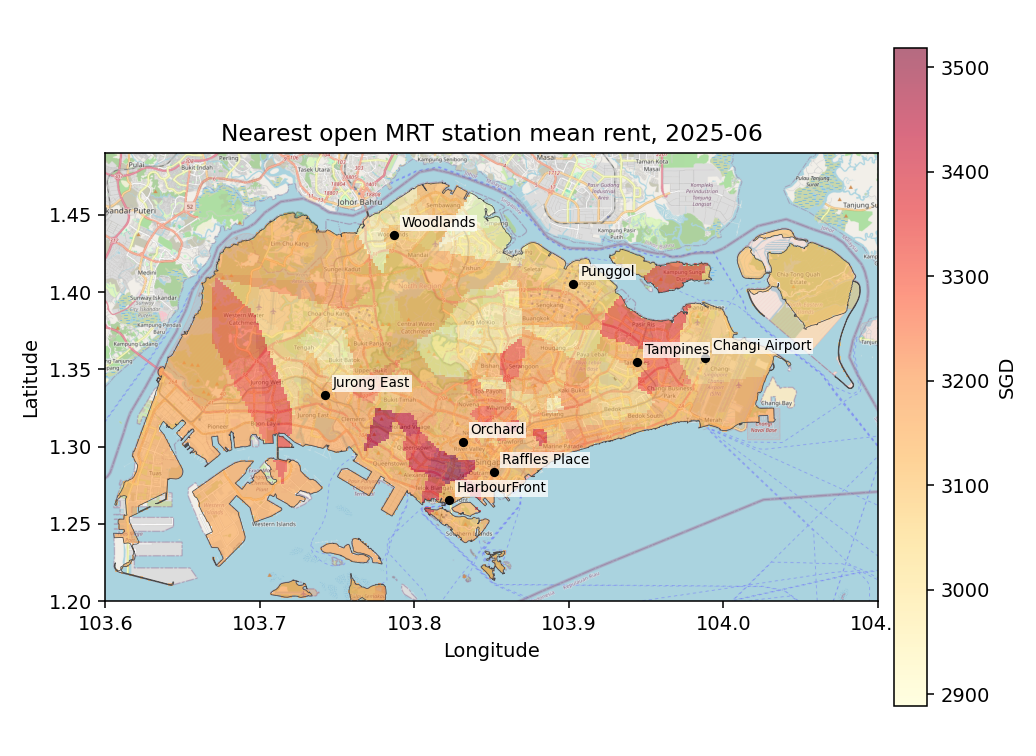
\includegraphics[width=0.92\linewidth]{../../outputs/figures/maps/map_mrt_2025-06.png}
\caption{Nearest open MRT station, June 2025.
Colour is the smoothed mean of labelled rents in the previous three months for that station.
Each area is one station.}
\label{fig:mrt-map}
\end{figure}

\subsection{Limits of the built columns}

\begin{itemize}
\item \texttt{MAX\_FLOOR} is the top floor of the block, not the flat's own floor.
Values of $-1$ on floor and completion year are sentinels and are stored as null (159 labelled rows, none in the private test set).
\item The MRT file has no opening date.
A station marked open may have opened after January 2021.
Planned stations and future-line prefixes are kept out of the open-station distance.
\item About 20 MRT longitudes have only one to three decimal places.
Switching from Haversine to SVY21 does not repair that.
\item Great-circle distance is not walking time.
School and mall tables have no opening dates, and the school table has no university.
\item COE and stock columns are constant within an approval month.
January 2021 COE lags are null because December 2020 is missing.
The property basket is missing on early labelled rows because one constituent starts later.
\item Group means are target encodings of the previous three months of labelled rents, not properties of a mall, station, or school.
January 2021 is null.
A mall mean covers rentals for which that mall is the nearest mall, not every flat inside a radius.
\item Empty postal codes (285 blocks) have no postal-sector group and fall back to that quarter's island-wide mean once the three-month window contains any labelled rent.
\end{itemize}

\section{Multistage model}
\label{sec:stack}

The scored model uses the columns above.
Figure~\ref{fig:stack} shows the path from those columns to a monthly rent.
Later tables report errors on the validation set and the test set.
Those sets, and the private test set, are defined in Section~\ref{sec:intro} and restated below.

\begin{figure}[ht]
\centering
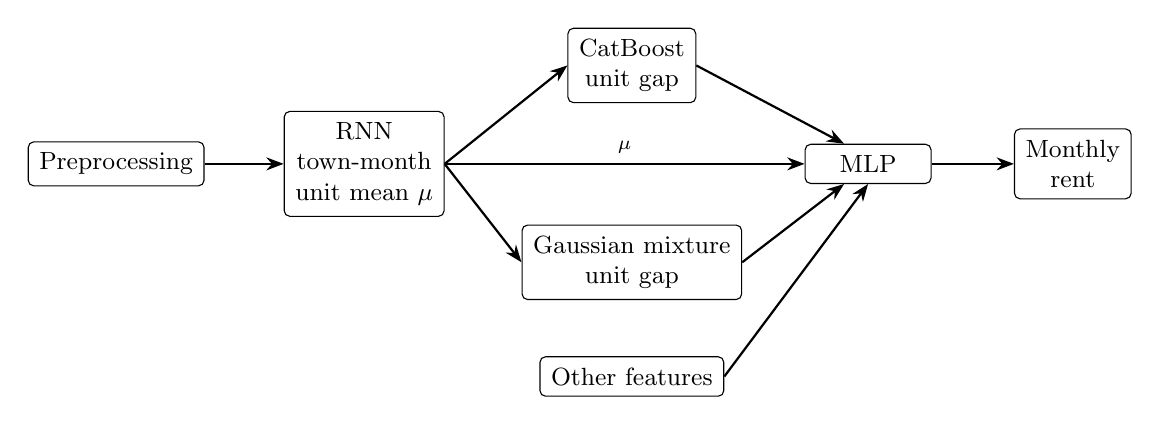
\begin{tikzpicture}[
  font=\small,
  box/.style={draw, rounded corners=2pt, align=center, inner sep=4pt},
  arr/.style={-{Stealth[length=2.2mm]}, thick}
]
\node[box] (prep) at (0,0) {Preprocessing};
\node[box] (rnn) at (3.15,0) {RNN\\town-month\\unit mean $\mu$};
\node[box] (cb) at (6.55,1.25) {CatBoost\\unit gap};
\node[box] (gmm) at (6.55,-1.25) {Gaussian mixture\\unit gap};
\node[box] (feat) at (6.55,-2.7) {Other features};
\node[box, minimum width=16mm] (mlp) at (9.55,0) {MLP};
\node[box] (out) at (12.15,0) {Monthly\\rent};
\draw[arr] (prep) -- (rnn);
\draw[arr] (rnn.east) -- (cb.west);
\draw[arr] (rnn.east) -- (gmm.west);
\draw[arr] (cb.east) -- (mlp.140);
\draw[arr] (gmm.east) -- (mlp.220);
\draw[arr] (rnn.east) -- node[above, font=\scriptsize] {$\mu$} (mlp.west);
\draw[arr] (feat.east) -- (mlp.south);
\draw[arr] (mlp) -- (out);
\end{tikzpicture}
\caption{Multistage prediction.
The RNN estimates the town-month rent per square metre.
CatBoost and the Gaussian mixture, fit separately, estimate the unit-price gap from that mean.
The MLP receives that mean, both gaps, and the flat's other features, and outputs monthly rent.}
\label{fig:stack}
\end{figure}

\subsection{Training, validation, test, and private test}

The labelled months are cut in time.
The training set is every approval month through September 2024, and it is the only set used to fit parameters.
The validation set is the next three months, October through December 2024, and it is the only set used to stop or choose a model.
The test set is the last three labelled months, January through March 2025.
It is scored after that choice and does not enter it.
The private test set is the unlabelled table after March 2025.
The preprocessor, the town coordinate scaling, and the mixture are fit on the training set only.

CatBoost's iteration and the network's epoch are the ones with the lowest validation RMSE under the patience rule.
The test set is a later quarter, kept so the report can say what happened after the choice, without letting that quarter make the choice.
The cut is by approval month, so the stopping decision cannot see leases from the test set.
Private-test RMSE is not used to stop or choose a model.

\subsection{Why the region is a town}

A partition trial compared five geographic units for a month mean.
Table~\ref{tab:cells} is the cell log on the training set.
Town has no missing rows.
A typical town-month cell has about 110 flats, and only 5.9\% of those cells have fewer than 30.
Planning areas are thinner, and postal districts and postal sectors also drop 4{,}685 rows that have no postal code.
Postal sectors then have a median of 34 rows, and 43.5\% of their cells are under 30.
Town is fine enough that towns differ, and still large enough that a typical cell is not a handful of leases.

\begin{table}[ht]
\centering
\caption{Cells in the training set for each geographic unit.
A cell is one unit in one approval month.
The share is the fraction of those cells with fewer than 30 flats.}
\label{tab:cells}
\begin{tabular}{lrrrrr}
\toprule
Unit & Groups & Missing rows & Cells & Median rows & Under 30 \\
\midrule
Region & 5 & 0 & 225 & 638 & 0\% \\
Town & 26 & 0 & 1{,}170 & 110.5 & 5.9\% \\
Planning area & 31 & 0 & 1{,}341 & 96 & 19.2\% \\
Postal district & 24 & 4{,}685 & 1{,}035 & 78 & 25.7\% \\
Postal sector & 53 & 4{,}685 & 2{,}261 & 34 & 43.5\% \\
\bottomrule
\end{tabular}
\end{table}

Table~\ref{tab:partition} scores a ridge of the town-month mean of \texttt{MONTHLY\_RENT}.
Town indicators plus a month index leave a large cell error.
Adding the category-C COE premium and the bank-basket level removes most of it.
Adding the property-basket level improves the next quarter further.
Using all 15 COE and stock columns, including changes, bid ratios, and returns, makes that quarter worse.
Month-to-month COE changes and bid ratios alone do not beat the month index.
The adopted economy inputs for the region mean are therefore the month index and those three level series.
A separate month slope for each town was worse than one shared slope.

\begin{table}[ht]
\centering
\caption{Weighted cell RMSE of the town-month mean of monthly rent, in SGD.
The validation set is October--December 2024.
The test set is January--March 2025 and did not choose the specification.}
\label{tab:partition}
\begin{tabular}{lrr}
\toprule
Specification & Validation & Test \\
\midrule
Town and month index & 291.65 & 366.09 \\
Plus COE C premium and bank basket & 94.37 & 112.85 \\
Plus property basket & 93.36 & 103.31 \\
All 15 COE and stock columns & 104.81 & 229.70 \\
\bottomrule
\end{tabular}
\end{table}

\subsection{Region mean}

The region model predicts the town-month mean of rent per square metre, monthly rent divided by floor area, with equal weight per flat.
Figure~\ref{fig:town-may} is one month of that quantity, May 2024.
The colour is the observed town mean, not a forecast.
Central and southern towns are darker than the north and west, so the town mean is not one island-wide number.
Each town has its own network.
The input is the time index and the economic trend from before the month being predicted.
The network does not see the true subsequent town-month rents.
The hidden state carries the earlier economic inputs.
Running the sequence from 2021 is required: a zero initial state would drop that history.

\begin{figure}[ht]
\centering
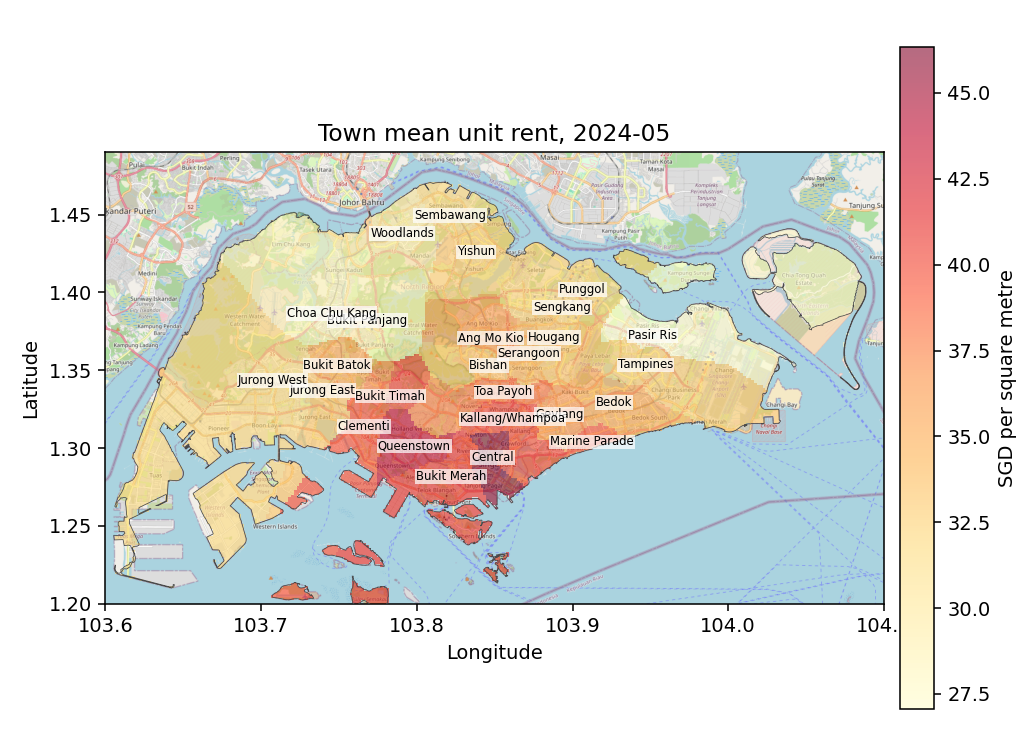
\includegraphics[width=0.92\linewidth]{../../outputs/figures/maps/town_unit_mean_2024-05.png}
\caption{May 2024 mean of rent per square metre by town.
Each patch is the town of the nearest HDB block.
The colour is the unweighted mean of the flats approved in that month.
The map was not scored.}
\label{fig:town-may}
\end{figure}

The network is an RNN with hidden size 16, three layers, and the default tanh nonlinearity, followed by a linear map from 16 units to one output.
It is trained for 50 epochs at learning rate 0.01 with seed 5228, on cells in the training set.
Weighted cell RMSE on the validation set is 0.9707 SGD per square metre.
On the test set it is 1.0897.
These are errors of the town-month unit-price mean, weighted by the number of flats in the cell.
They are not the flat-level RMSE of monthly rent, and they are not mean squared error.
They also cannot be compared with a cell RMSE computed on monthly rent in dollars.

Earlier trials on the dollar town-month mean are a different target.
Among them, a one-layer RNN had validation cell RMSE 93.25 and test cell RMSE 88.04, and its cross-town mean on the private test set moved from 3192 in April 2025 to 3274 in July 2026.
A four-input three-layer LSTM had validation cell RMSE 88.75 and test cell RMSE 83.39, but its private-test path fell slightly, from 3132 to 3109.
A linear bypass beside that LSTM fit the cells, with training-set cell RMSE 83.73, and then overshot: validation cell RMSE 170.56, test cell RMSE 261.29, and a private-test path from 3339 to 3821.
On the unit-price target, a linear-bypass LSTM scored 1.9646 and 3.4044.
The three-layer per-square-metre RNN is the region mean used by the stack.
Its cross-town unit mean on the private test set goes from 35.99 in April 2025 to 35.79 in July 2026.
Test-set cell RMSE did not choose the network.

\subsection{A within-town surface}

Figure~\ref{fig:bukit} is Bukit Panjang, drawn from the saved stack mixture rather than from the all-label refit.
The six components in the title are the number that town kept.
The colour scale is shared across towns, symmetric about zero, at the 98th percentile of absolute values.
A cell more than 400\,m from a flat in the training set is blank.
The figure was not chosen by RMSE.

The surface is the mixture's conditional per-square-metre gap, evaluated at that town's mean flat-type rank and mean flat-model rank.
It is the predicted gap from the region mean, not the rent itself.
December 2024 points are that month's unit rent minus Bukit Panjang's true December unit mean.
The annotation states those two December means: the true mean is 30.19 SGD per square metre, and the RNN region mean is 30.71.
A point and the cell under it do not use the same baseline.
The point uses the true December mean.
The surface uses the predicted gap from the region mean.

\begin{figure}[ht]
\centering
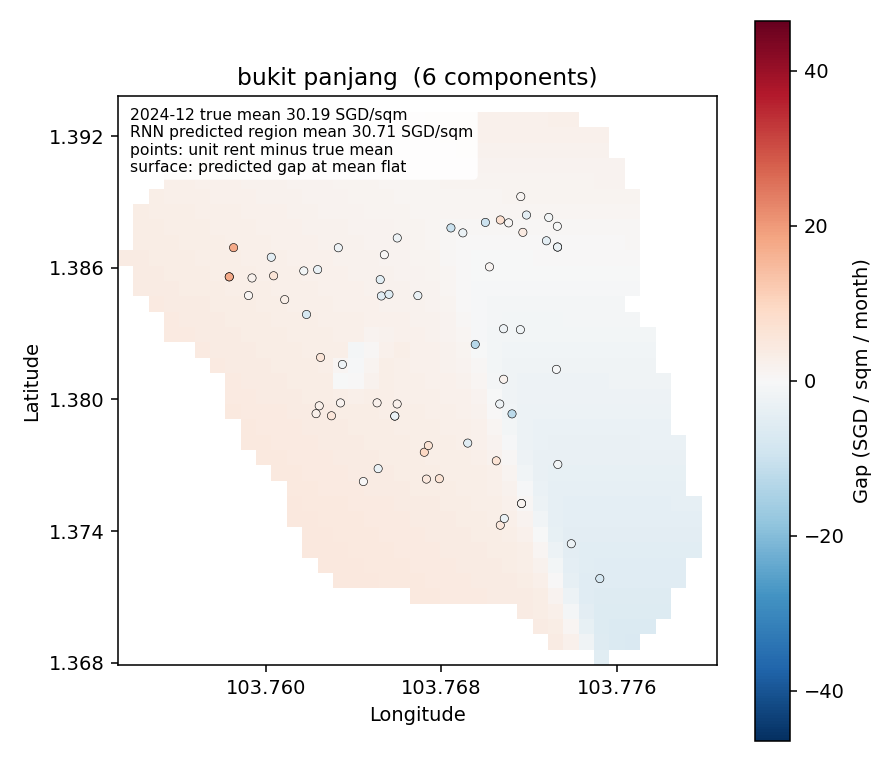
\includegraphics[width=0.86\linewidth]{../../src/viz/gaussian_towns/bukit_panjang.png}
\caption{Bukit Panjang.
The surface is the conditional per-square-metre gap at the town's mean flat ranks.
December 2024 points are unit rent minus that town's true December unit mean.
Cells farther than 400\,m from a flat in the training set are blank.}
\label{fig:bukit}
\end{figure}

\subsection{Within-town gap}

CatBoost and a Gaussian mixture are fit separately, one pair per town, to the same target: unit rent minus the RNN town-month unit mean.
Neither model sees the other's output.
CatBoost is used because the within-town columns include names and codes, and a tree can split on a subset of those names.
The mixture is used because the remaining gap still varies smoothly with where the flat sits inside the town.
Both are then turned back into a monthly-rent error by adding the gap to the RNN mean and multiplying by floor area.
Table~\ref{tab:gap} records those errors.
RMSE on the test set did not choose either model.

\begin{table}[ht]
\centering
\caption{RMSE after adding the predicted gap to the RNN unit mean.
The rent columns multiply that unit price by floor area.
The test set did not choose the model.}
\label{tab:gap}
\begin{tabular}{lrrrr}
\toprule
 & \multicolumn{2}{c}{SGD per square metre} & \multicolumn{2}{c}{Monthly rent, SGD} \\
\cmidrule(lr){2-3}\cmidrule(lr){4-5}
Model & Validation & Test & Validation & Test \\
\midrule
CatBoost & 5.3811 & 5.4562 & 455.06 & 469.19 \\
Mixture & 5.7707 & 5.8380 & 490.02 & 502.48 \\
\bottomrule
\end{tabular}
\end{table}

The town CatBoost uses depth 8, learning rate 0.05, at most 1000 iterations, and early stopping of 50 rounds on the validation set.
Its columns are fixed: latitude and longitude; block and street keys; flat-type rank, flat-model rank, and flat-model name; nearest open MRT code, distance, and log distance; nearest mall name and distance; and nearest primary and secondary names and distances.
Categories stay native.
Numeric columns are median-imputed and are not scaled.
A rare level needs 30 rows.
An unseen category becomes a missing token.

This list is not the feature set produced by ablation.
The production pipeline starts each model on the ten source columns, then probes auxiliary columns one at a time.
For CatBoost a probe is promising only when its validation RMSE is strictly lower than that round's current set.
The current columns plus every promising column replace the saved set only when their own validation RMSE is lower.
A later stage retrains the columns already kept, with a larger budget, and does not add or drop columns.
The columns that process kept are a different 40-column CatBoost, including several line-specific station fields and five of the group-mean rents.
That model is not the town stage, and the stack does not replace it.

\subsection{Mixture assumptions}

Each town's mixture is a full-covariance Gaussian mixture in five dimensions: latitude and longitude standardized inside the town, flat-type rank and flat-model rank standardized inside the town, and the per-square-metre residual.
The residual is a coordinate.
It is allowed to be negative, so a component can sit below the region mean as well as above it.
The prediction is the responsibility-weighted conditional mean of that residual given the location and the two ranks.
It is not a probability multiplied by the region mean.
The component count starts at 20.
If any component that is hard-assigned on the training set has fewer than 30 rows, the count drops by one and the town is refit, down to one component.
Bukit Panjang kept 6.
Across towns the kept counts in the scored training run from 3 to 19.

An earlier location check, on a dollar gap rather than this five-dimensional unit-price mixture, is what was validated.
Across 76 components, the training-set dollar gap and the validation-set gap correlate 0.890, with mean absolute error 69.1.
An own-town surface starting at three components has validation row RMSE 578.11 and test row RMSE 593.19.
A density blend across towns is worse, at 579.76 and 594.42.
Starting the own-town surface at 10, with the same drop rule, scores validation row RMSE 566.55 and test row RMSE 580.58.
That correlation was not recomputed for the current per-square-metre mixture.
The current mixture is scored by the rent RMSE in Table~\ref{tab:gap}.

\subsection{The shared network}

One network sees every town.
It is not trained separately by town.
The town-specific pieces it receives are the RNN mean, the CatBoost gap, and the mixture gap.
The network has a linear map to 128 units, a ReLU, dropout 0.1, a linear map to 64 units, a ReLU, dropout 0.1, and a linear map to one output.
Optimization is Adam with learning rate 0.001 and batch size 1024.
The target is monthly rent, standardized on the training set and restored before the error is computed.
The output is monthly rent.
Area is not applied again after the network.

The 27 inputs are the RNN unit mean, the CatBoost unit gap, the mixture unit gap, and floor area, each as its own column; fee; lease commencement year; building age; month index; latitude and longitude after within-town standardization; raw latitude and longitude in degrees; flat-type rank; flat-model rank; maximum floor; year completed; flat age from the lease; distances to the nearest open MRT, mall, primary school, and secondary school; the log MRT distance; and counts of open MRT stations, malls, primary schools, and secondary schools within 1\,km, plus other HDB blocks within 500\,m.

Training runs for at most 100 epochs.
After each epoch the validation RMSE of monthly rent is computed.
If that RMSE does not fall by more than $10^{-6}$ for 10 consecutive epochs, training stops and the weights from the best validation epoch are restored.
Test RMSE is computed after that choice and does not enter it.
The kept run stops at epoch 8.
Validation RMSE is 448.24.
Test RMSE is 462.87.
Training RMSE on the training set is 461.25.
The CatBoost gap on the training set is the saved full model's prediction on its own training rows, because out-of-fold vectors were not stored.
Validation, test, and private-test CatBoost features are that same full model applied to those rows.

A wider network, with widths 512, 256, 128, and 64, dropout 0.3, and patience 40, was tried on an earlier dollar region mean.
Its validation RMSE was 448.88 and its test RMSE was 461.87 at epoch 29.
It is not the stack prediction.
That validation RMSE belongs to a different region mean and is not a comparison with 448.24.

\section{Conclusion}
\label{sec:conclusion}

The submitted prediction is the multistage model of Section~\ref{sec:stack}: a town-month unit-price mean, two within-town gaps from that mean, and one shared network.
Validation RMSE of monthly rent is 448.24 and test RMSE is 462.87.
The test set did not make the choice.
Figure~\ref{fig:kaggle} records the score on the private test set.
The latest submission has RMSE 451.26.

\begin{figure}[ht]
\centering

\includegraphics[width=\linewidth]{kaggle_leaderboard.png}
\caption{Private test set.
Gold Miner (Group 12) is ranked 43 after six submissions.
The latest submission scores 451.26, against a previous best of 453.16.}
\label{fig:kaggle}
\end{figure}

The RNN hidden state uses tanh, so the region mean cannot grow without a bound.
On the private test set its cross-town unit-price mean stays near 35.99 in April 2025 and 35.79 in July 2026.
A linear bypass can keep a slope past the training set, but the comparisons that were run favoured the RNN.
On the dollar town-month mean that bypass overshot, with validation cell RMSE 170.56, while the one-layer RNN, from 3192 to 3274, stayed closest to the external approved-rent path of about 3179 to 3280.
The three-layer per-square-metre RNN is the region mean in the scored model.

\end{document}
